\begin{frame}{Contrôle de la respiration}
	\centering
	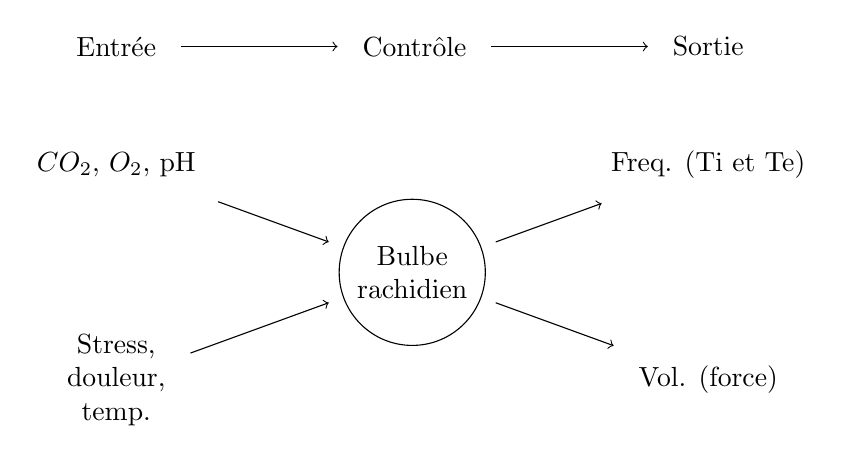
\begin{tikzpicture}[
			outer sep=2mm,
			bulbe rachidien/.style={
			draw,
			circle,
			align=flush center
		}
		]

		\node [bulbe rachidien] (cr) {Bulbe\\rachidien};

		\node (co2) at(160:4) {$CO_2$, $O_2$, pH};
		\node [align=flush center] (cortex) at(200:4) {Stress,\\douleur,\\temp.};
		\node (freq) at(20:4) {Freq. (Ti et Te)};
		\node (vol) at(-20:4) {Vol. (force)};

		\node [yshift=1.5cm] (E) at (co2) {\structure{Entrée}};
		\node [yshift=1.5cm] (S) at (freq) {\structure{Sortie}};
		\path (E) -- (S) node [midway] (C) {\structure{Contrôle}} ;

		\draw [->] (E) -- (C);
		\draw [->] (C) -- (S);
		\draw [->] (co2) -- (cr);
		\draw [->] (cortex) -- (cr);
		\draw [->] (cr) -- (freq);
		\draw [->] (cr) -- (vol);
	\end{tikzpicture}
\end{frame}

\begin{frame}{Contrôle de la respiration}
	\centering
	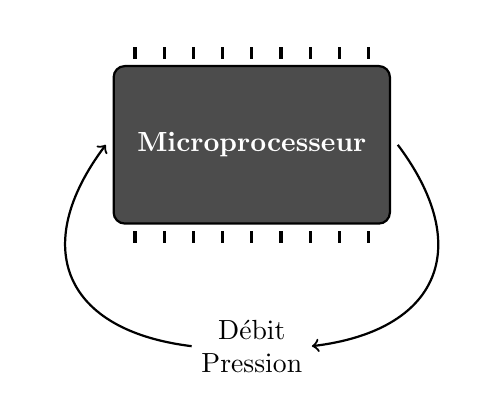
\begin{tikzpicture}[
			pin distance=1ex,
			every pin edge/.style={
				very thick
			},
			cpupin/.style={
				inner sep=0
			},
			cpu/.style={
				thick,
				draw, 
				rounded corners, 
				outer sep=1mm,
				minimum size=2cm,
				fill=black!70,
				text=white,
				inner sep=3mm,
				font=\bf,
				append after command={
					(CPU.150) -- (CPU.30) 
					foreach \dist in {1, 2, ..., 9}{%
						node[cpupin, pos=0.1*\dist, pin={90:{}} ] (P\dist) {}
						}
						(CPU.-150) -- (CPU.-30) 
						foreach \dist in {1, 2, ..., 9}{%
							node[cpupin, pos=0.1*\dist, pin={-90:{}} ] (P\dist) {}
							}
						}
					},
					arklink/.style={
						bend left=60,
						->,
						looseness=1.5,
						thick
					}
				]

		\node [cpu] (CPU) {Microprocesseur};
		\node [below=1cm, align=flush center] (E) at(CPU.south) {Débit\\Pression};
		\draw[arklink] (CPU.east) to (E.east);
		\draw[arklink] (E.west) to (CPU.west);
		%\node [left=1cm] (E) at(CPU.west) {Débit, Pression};
		%\node [right=1cm] (O) at(CPU.east) {Débit, Pression};
		%\draw [->] (E) -- (CPU);
		%\draw [->] (CPU) -- (O);


	\end{tikzpicture}
\end{frame}
